\documentclass[11pt,a4paper]{report}

%https://tex.stackexchange.com/questions/134079/font-setup-for-an-academic-thesis-no-computer-modern-wanted
%\usepackage[libertine,cmintegrals,cmbraces,vvarbb]{newtxmath}
%\usepackage[scaled=0.95]{inconsolata}
%\usepackage{classicthesis}
\usepackage[sc]{mathpazo}

%\usepackage{helvet}
%\renewcommand{\familydefault}{\sfdefault}

\linespread{1.1}
\usepackage[margin=1in]{geometry}

\usepackage[sort,numbers,sectionbib]{natbib}
%\usepackage{natbib}
%\usepackage{biblatex}
\bibliographystyle{IEEEtran}
\renewcommand{\bibname}{References}

% http://ctan.org/pkg/lipsum
\usepackage{lipsum}

% https://tex.stackexchange.com/questions/94224/how-to-create-a-list-with-a-fixed-prefix-and-incremental-numbers
\usepackage{enumitem}

% https://tex.stackexchange.com/questions/86120/font-size-of-figure-caption-header
\usepackage[font=scriptsize,labelfont=bf]{caption}

%https://tex.stackexchange.com/questions/3001/list-sections-of-chapter-at-beginning-of-that-chapter
% !!! NEEDS TO BE ABOVE HYPEREF !!!
\usepackage{titletoc}

% https://www.sharelatex.com/learn/Hyperlinks
\usepackage{hyperref}
\hypersetup{
    colorlinks,
    %citecolor=gray,
    citecolor=blue,
    filecolor=black,
    linkcolor=blue,
    urlcolor=blue,
    linktoc=all
}

% includegraphics
\usepackage[]{graphicx}
\graphicspath{{img/}}
\usepackage{mwe}


\usepackage[outputdir=build]{minted}
%https://www.sharelatex.com/learn/Code_Highlighting_with_minted#Reference_guide
\usemintedstyle{vs}
% https://tex.stackexchange.com/questions/161124/how-to-make-a-minted-code-listing-centered-on-a-page
%\RecustomVerbatimEnvironment{Verbatim}{BVerbatim}{}

% tables, row colour
\usepackage{tabularx,colortbl,booktabs}
% For vertical centering text in X column
\renewcommand\tabularxcolumn[1]{m{#1}}
\def\arraystretch{1.3}

\begin{document}
%TC:ignore
\pagestyle{headings}

\begin{titlepage}
\begin{center}

\vspace*{2cm}
\Large

\textbf{
%%PRCO304 - Project Initiation Document
%Highlight Reports
Multi-core RISC Processor Design and Implementation (Rev. 1.00)
}

\vspace{0.4cm}
\large
%%Space optimised FPGA-based side-microprocessor.
ELEC5881M - Interim Report
%%EMBEDDED CPU - FPGA-based RISC microprocessor

\vspace{2cm}
\textbf{Ben David Lancaster}\\
Student ID: 201280376

\vspace{2cm}
Submitted in accordance with the requirements for the degree of\\
Master of Science (MSc)\\
in Embedded Systems Engineering\\

\vspace{2cm}
Supervisor: Dr. David Cowell\\
Assessor: Mr David Moore

\vspace{2cm}
\textbf{University of Leeds}\\
School of Electrical and Electronic Engineering

\vspace{2cm}
\today
\end{center}
\end{titlepage}

%\newpage
%\chapter*{Abstract}
%\lipsum[1-3]

\newpage
\section*{Revision History}
\begin{table}[h]
\def\arraystretch{1.3}
    \begin{tabularx}{\textwidth}{|l|l|X|}
    \hline
    Date & Version & Changes \\
    %\arrayrulecolor{\color{red}}
	\specialrule{2pt}{-2pt}{0pt}
	10/04/2019 & 2.01 & Add introduction. \\ \hline
	05/04/2019 & 2.01 & Fix processor RTL diagram. \\ \hline
	04/04/2019 & 2.00 & Initial processor RTL diagram. \\ \hline
	01/04/2019 & 1.00 & Initial section outline. \\ \hline
    \end{tabularx}
    \caption{Document revisions.}
\end{table}

%\newpage
%\chapter*{Acknowledgements}
%I would like to thank my project supervisor Dr David Cowell for their support and guidance throughout this project.


\chapter*{Declaration of Academic Integrity}
%\addcontentsline{toc}{chapter}{Declaration of Academic Integrity}

The candidate confirms that the work submitted is his/her own, except where work which has formed part of jointly-authored publications has been included. The contribution of the candidate and the other authors to this work has been explicitly indicated in the report. The candidate confirms that appropriate credit has been given within the report where reference has been made to the work of others.

This copy has been supplied on the understanding that no quotation from the report may be published without proper acknowledgement. The candidate, however, confirms his/her consent to the University of Leeds copying and distributing all or part of this work in any forms and using third parties, who might be outside the University, to monitor breaches of regulations, to verify whether this work contains plagiarised material, and for quality assurance purposes.

The candidate confirms that the details of any mitigating circumstances have been submitted to the Student Support Office at the School of Electronic and Electrical Engineering, at the University of Leeds.
\vfill

\noindent 
Name: Ben David Lancaster \\
Date: \today
\newpage


\newpage
\renewcommand*\contentsname{Table of Contents}
{%\hypersetup{linkcolor=black}
\tableofcontents
%\listoffigures
%\listoftables}
%TC:endignore

\newpage
\chapter{Introduction}
{%\hypersetup{linkcolor=black}
\startcontents[chapters]
\printcontents[chapters]{}{1}{}
}

\noindent\\
Moore's Law states that the number of transistors in a chip will double every 2 years \cite{}. CPU designers would utilize the  additional transistors to add more pipeline stages in the processor to reduce the propagation delay \cite{}. This would allow the processor to be run at higher clock frequencies as the logic between pipeline stages is reduced. The faster clock frequency would result in computational performance because more instructions could be executed in a period of time.

The size of transistors have been decreasing \cite{} and today can be manufactured in sub-10 nanometer range. However, the extremely small transistor size increases electrical leakage and other negative effects resulting in unreliability and potential damage to the transistor \cite{}.  The high transistor count produces large amounts of heat and requires increasing power to supply the chip. These trade-offs are currently managed by reducing the input voltage, utilising complex cooling techniques, and reducing clock frequency. These factors limit the performance of the chip significantly.
These are contributing factors to Moore's Law \textit{slowing} down.

The capacity limit of transitional planar transistors is approaching and so in order for performance increases to continue, other approaches such as alternate transistor technologies like Multigate transistors \cite{subramanian2010multiple}, software and hardware optimisations, and multi-processor architectures are employed.

\section{Why Multi-core?}
This report will focus on the latter approach: to design, implement, and verify a new multi-core RISC processor, with an emphasis on multi-core communication techniques.

 

\section{Why RISC?}
RISC architectures 

\section{Why FPGA?}
    
\chapter{Background}
{%\hypersetup{linkcolor=black}
\startcontents[chapters]
\printcontents[chapters]{}{1}{}
}
\noindent\\
Testing

\section{Single core vs. Multi-core vs. Many-core}
\section{Network-on-chip}
Network-on-chip (NoC) architectures implement on-chip communication mechanisms that are based on network communication  principles, such as routing, switching, and massive scalability.

\subsection{OpenPiton}
\section{Summary}
    
\chapter{Project Overview}
{%\hypersetup{linkcolor=black}
\startcontents[chapters]
\printcontents[chapters]{}{1}{}
}
\noindent\\
This chapter discusses the the project's requirements, goals, risks, and structure.

\section{Project Deliverables}
The project's deliverables are split into two sections: core deliverables (CD) -- each deliverable must be satisfied for the project to be a minimum viable product (MVP), and extended deliverables (ED) -- deliverables that are not required for a MVP -- features that only improve upon an existing feature.

\subsection{Core Deliverables (CD)}
The project's core deliverables are described below.
\begin{enumerate}[leftmargin=2\parindent, label=\bfseries CD\arabic*]
    \item{Design a compact 16-bit RISC instruction set architecture.}\label{cd:isa}
    \item{Design and implement a Verilog RISC core that implements the ISA in \ref{cd:isa}.}\label{cd:core}
    \item{Design and implement an on-chip interconnect for multi-core processing (2 to 32 cores) using the RISC core from \ref{cd:core}.}\label{cd:interconnect}
    \item{Analyse performance of serial and parallel software algorithms, such as parallel DFT \cite{dft}, on the processor.}\label{cd:software}
    \item{Allow the RISC core to be easily compiled to multiple FPGA vendors (Xilinx, Altera).}\label{cd:vendor}
\end{enumerate}

\subsection{Extended Deliverables (ED)}
The project's extended deliverables are described below.
\begin{enumerate}[leftmargin=2\parindent, label=\bfseries ED\arabic*]
    \item{Design a RISC core with an instructions-per-clock (IPC) rating of at least 1.0 (a single-cycle CPU).}\label{ed:ipc}
    \item{Design a RISC core with a pipe-lined data path to increase the design's clock speed.}\label{ed:pipeline}
    \item{Design a scalable multi-core interconnect supporting arbitrary (more than 32) RISC core instances (manycore) using Network-on-Chip (NoC) architecture.}\label{ed:scale}
    \item{Design a compiler-backend for the PRCO304 \cite{prco304} compiler to support the ISA from1 \ref{cd:isa}. This will make it easier to build complex multi-core software for the processor.}\label{ed:compiler}
    \item{The RISC core can communicate to peripherals via a memory-mapped addresses using the Wishbone \cite{wishbone} bus.}\label{ed:mmu}
    \item{Implement various memory-mapped peripherals such as UART, GPIO, LCD, to aid visual representation of the processor during the demonstration viva.}\label{ed:peripherals} 
    \item{Store instruction memory in SPI flash.}\label{ed:flash}
    \item{Reprogram instruction memory at runtime from host computer.}\label{ed:program}
    \item{Processor external debugger using host-processor link.}\label{ed:debug}
\end{enumerate}

\section{Project Timeline}\label{sect:timeline}
\subsection{Project Stages}
The project is split up into many stages to aid planning and management of the project. There are 8 unique stage areas: 1. Inital project conception; 2 Basic RISC core development; 3. Extended RISC core development; 4. Multi-core development; 5. Processor quality-of-life (QoL) improvements; 6. Compiler development; 7. Demo preparation, and 8. Final report.

The project stages are shown in Table \ref{tb:stages}.

\begin{table}[h]
    \small
    \begin{tabularx}{\textwidth}{|l|l|l|l|l|X|}
    \hline
    Stage & Title & Start Date & Days & Core & Applicable Deliverables
    \\ \specialrule{2pt}{-2pt}{0pt}
    1.0 & Research & Feb 04 & 7 & x & 
    \\ \hline
    1.1 & Requirement gathering/review & Feb 11 & 14 & x & 
	\\ \hline
    1.1 & Processor specification, architecture, ISA & Feb 18 & 100 & x & \ref{cd:isa}
	\\ \hline
    1.2 & Stage/Time Allocation Planning & Feb 25 & 7 & x & 
    \\ \specialrule{2pt}{-2pt}{0pt}
    2.1 & Decoder, Register Set, impl \& integration & Feb 25 & 14 & x & \ref{cd:core}
	\\ \hline
    2.2 & Register set impl \& integration & Mar 04 & 14 & x & \ref{cd:core}
	\\ \hline
    2.3 & Local memory impl \& integration & Mar 11 & 14 & x & \ref{cd:core}
    \\ \specialrule{2pt}{-2pt}{0pt}
    3.1 & Memory mapped register layout \& impl & Apr 01 & 21 &  & \ref{ed:mmu}
	\\ \hline
    3.2 & Wishbone peripheral bus connected to MMU & Apr 08 & 21 &  & \ref{ed:mmu}
	\\ \hline
    3.3 & Pipelined implementation and verification & Apr 15 & 21 &  & \ref{ed:pipeline}
	\\ \hline
    3.4 & Cache memory design \& impl & Apr 22 & 28 &  & \ref{ed:pipeline}
    \\ \specialrule{2pt}{-2pt}{0pt}
    4.1 & Multi-core communication interface & TBD & TBD & x & \ref{cd:interconnect}
	\\ \hline
    4.2 & Shared-memory controller & TBD & TBD & x & \ref{cd:interconnect}
	\\ \hline
    4.3 & Scalable multi-core interface (10s of cores) & TBD & TBD & x & \ref{cd:interconnect}
	\\ \hline
    4.4 & Multi-core example program (reduction) & TBD & TBD & x & \ref{cd:software}
    \\ \specialrule{2pt}{-2pt}{0pt}
    5.1 & SPI-FPGA interface for OTG programming & TBD & TBD &  & \ref{ed:flash}
	\\ \hline
    5.2 & FPGA-PC interfacing & TBD & TBD &  & \ref{ed:debug}
	\\ \hline
    5.3 & FPGA-PC debugging (instruction breakpoints) & TBD & TBD &  & \ref{ed:debug}
    \\ \specialrule{2pt}{-2pt}{0pt}
    6.1 & Compiler backend for vmicro16 & TBD & TBD &  & \ref{ed:compiler}
	\\ \hline
    6.2 & Compiler support for multi-core codegen & TBD & TBD &  & \ref{ed:compiler}
    \\ \specialrule{2pt}{-2pt}{0pt}
    7.1 & Wishbone peripherals for demo & TBD & TBD & x & \ref{cd:software}
    \\ \specialrule{2pt}{-2pt}{0pt}
    8.1 & Final Report & TBD & TBD & x & 
	\\ \hline
    \end{tabularx}
    \caption{Project stages throughout the life cycle of the project.}
    \label{tb:stages}
\end{table}

\subsection{Timeline}
The project stages from Table \ref{tb:stages} are displayed below in a Gantt chart.

\begin{figure}[h]
\centering
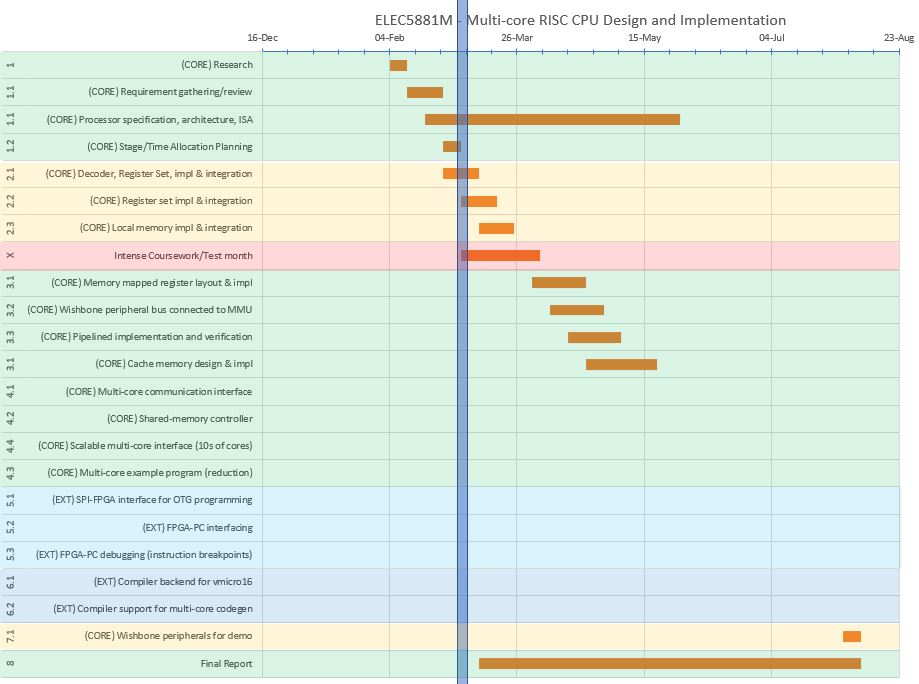
\includegraphics[width=13cm]{../img/week1_gantt}
\label{fig:arduino_record}
\caption{Project stages in a Gantt chart.}
\end{figure}


\section{Resources}
This section describes the hardware and software resources required to design and implement the project. 

\subsection{Hardware Resources}
Core deliverable \ref{cd:vendor} requires the designed RISC core to be implemented and demonstrated on multiple FPGA devices.  Although my design should synthesise for physical IC implementation, due to high costs and lengthy production times, it is not a primary development target.

Due to having past experience with Xilinx FPGAs from my placement work and experience with Altera from university modules it was decided to target the Xilinx Spartan 6 XC6SLX9 and the Altera Cyclone V.

\subsubsection{Terasic DE1-SoC Development Board}
The Terasic DE1-SoC development board features a large Cyclone V FPGA and many peripherals, such as seven-segment displays, 64 MB SDRAM, ADCs, and buttons and switches, which will aid demonstration of the project. The development board is available through the university so the cost is negligible. Figure \ref{fig:de1soc} shows the peripherals (green) available to the FPGA.

\begin{figure}[h]
\centering 
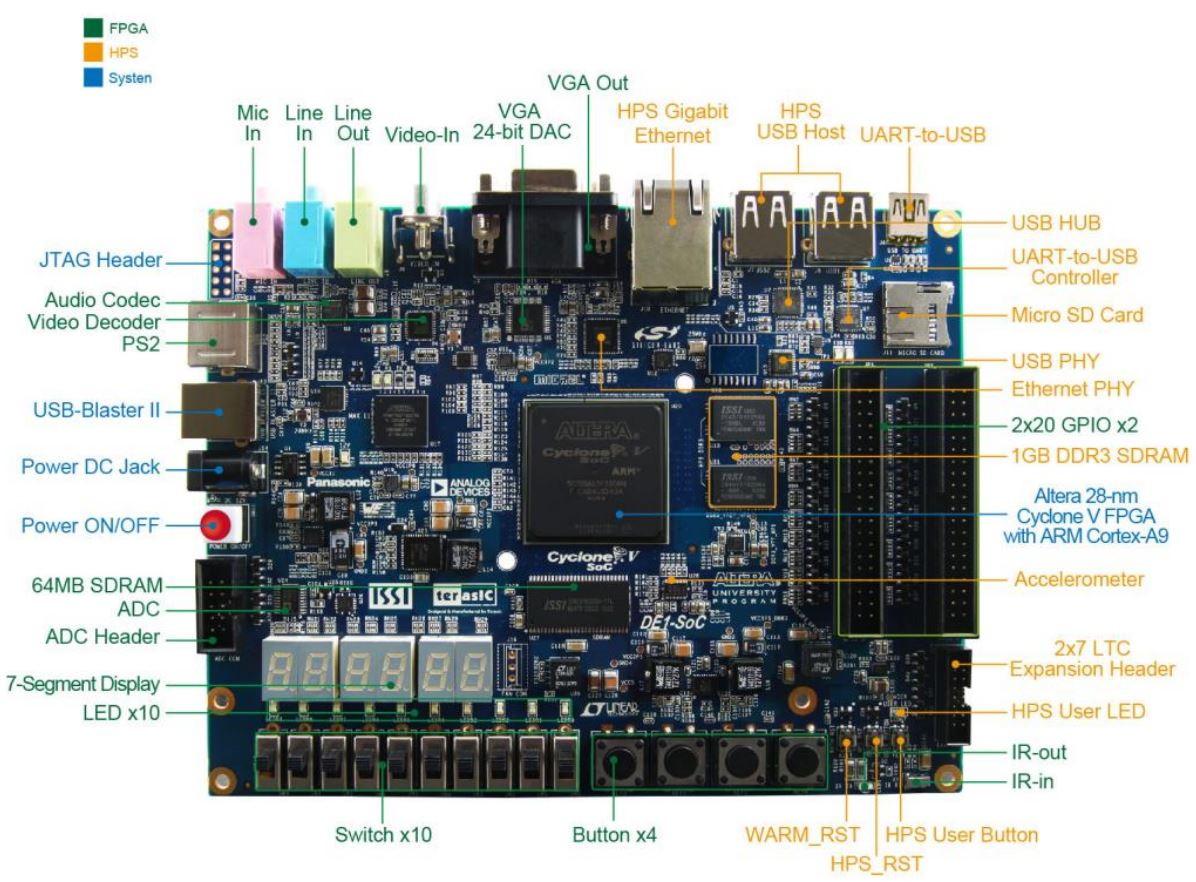
\includegraphics[width=10cm]{../img/de1soc}
\caption{Terasic DE1-SoC development board featuring the Altera Cyclone V FPGA and many peripherals. Image source: \cite{de1soc}.}
\label{fig:de1soc}
\end{figure}

\subsubsection{Minispartan 6+ FPGA Development Board}
The Minispartan 6+ is a hobbyist FGPA development board with fewer peripherals than the DE1-SoC. The board's simplicity will ease debugging. The board features a Xilinx Spartan 6 XC6LX9 however it's simplicity and Xilinx's software suite will speed up development.

\begin{figure}[h]
\centering 
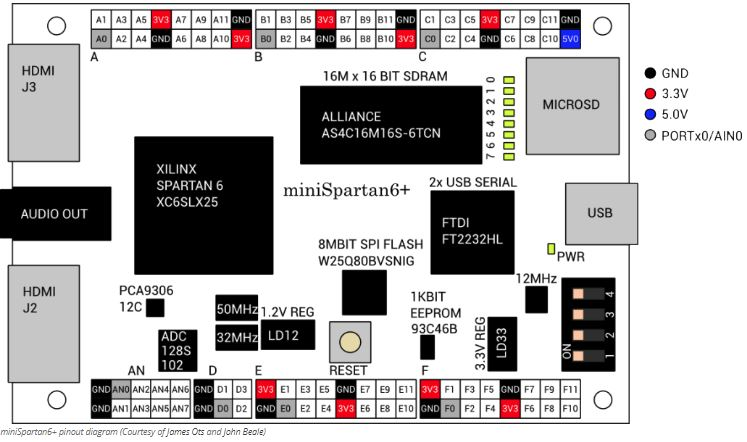
\includegraphics[width=10cm]{../img/minispartan}
\caption{Minispartan-6+ development board featuring the Xilinx Spartan 6 XC6SLX9. Image source: \cite{scarabhardware}.}
\label{fig:minispartan}
\end{figure}

\subsection{Software Resources}
\subsubsection{Intel Quartus}
Intel Quartus Prime is a paid-for SoC, CPLD, and FPGA software suite targeting Intel's Stratix, Arria, and Cyclone based FPGAs. The university provides student licences which will be used via VPN.


\subsubsection{Xilinx ISE Webpack}
Xilinx ISE Webkpack is Xilinx's free software suite for FPGA development for Spartan 6 based FPGAs.
Due to ISE's intuitive and fast work flow, most of the initial simulation and verification processes will be performed using ISE. This will greatly improve development times.

\subsubsection{Verilator}
Verilator is an open-source Verilog to C++ transpiler which provides a C++ interface to simulate Verilog modules and read/write values similar to a test bench. Verilator will be used for specific modules within the RISC core such as the ALU and decoder as Verilator is useful when performing exhaustive verification.

\section{Legal and Ethical Considerations}
The RISC core is designed to be used as an academic research and educational tool to aid learning and understanding of RISC and multi-core machines. It should not be use for roles where mission critical or safety is a factor. 

The processor does not provide any memory protection features and any software running on the processor has full access to all memory.

The processor does not store/track/predict software instructions. The processor uses pipelining techniques to improve performance which results in future instructions entering the pipeline even if the software's logical sequence does not include said instructions. This could result in security vulnerabilities similar to Intel's Spectre vulnerability \cite{kocher2018spectre}.


\chapter{Current Progress}
{%\hypersetup{linkcolor=black}
\startcontents[chapters]
\printcontents[chapters]{}{1}{}
}
\noindent\\
This chapter discusses the current progress made towards the project, including designs, implementation, and current results.

\section{RISC Core}
Following the project time line described in section \ref{sect:timeline}, the first couple months have been dedicated to the design and implementation of the instruction set architecture and RISC core with stages 1-3. Good progress has been made in both deliverables, the ISA and the RISC core, and the progress is on-time with the initial project time line.

\subsection{Instruction Set Architecture}
A 16-bit instruction set architecture (ISA) has been designed using an iterative approach. There currently exists 32 unique instructions covering most generic RISC operations (add, load/store, branch, compare, etc.) and atleast 16 opcodes available to be provide multi-core communication and functionality. This number should be adequate to support these features when the work begins on the multi-core project stages (stages 4-7).

\subsubsection{Design Goals}
Having past experience designing and implementing ISAs for previous projects, I wanted to use that knowledge to design an even more efficient and compact instruction set that could provide much greater functionality. The technical design goals of the ISA are described below:

\begin{enumerate}[leftmargin=3\parindent, label=\bfseries ISA\arabic*, style=nextline]
\item{\textbf{Use a fixed width of 16-bits for all instructions.}\\
This will significantly reduce RTL resources and encourage efficiency by not wasting spare bits. In addition, many SPI flash and RAMs support 16-bit wide data reads which will allow each instruction fetch to only require one clock cycle, thus increasing processor performance.}\label{isa:16}

\item{\textbf{Be able to select at least two registers for common instructions.}\\
This will reduce the number of required instructions to manipulate register data. A disadvantage of using two instead of three reigster selects is that instructions are always destructive -- they always \textit{destroy} existing data in the destination register (e.g. R0 = ADD R0 R1) unlike constructive instructions that provide a unique register select for the destination (e.g. R2 = ADD R0 R1). }\label{isa:regs}

\item{\textbf{Reduce bit-space for frequently used instructions (MOV, MOVI, ADD).}\\
Due to the 16-bit limit, two register selects, and immediate values, the opcode bits are reduced resulting in fewer unique instructions. To overcome this constraint, spare bits in other instructions will be appended to the opcode bits to extend the opcode range. This however, will require a more complex decoder that must first switch the opcode, then switch any spare bits to determine the final opcode. This method will significantly increase the number of unique instructions provided by the instruction set.}\label{isa:bits}

\item{\textbf{Provide frequently used actions as options for existing instructions.}\\
In software, frequently used actions include incrementing/decrementing by 1 and performing logical comparisons which usually take more than one instruction on some RISC architectures. As they are common actions, the instruction overhead and time may be significant and can affect performance. To provide a solution to this problem, in addition to using spare bits to extend the opcode range, spare bits will be used to signify a frequently used action action to be performed by the ALU.

As shown in Figure \ref{fig:isa}, frequently used commands such as incrementing/decrementing and logical comparions are provided by setting spare bits to special values. For example, the instructions \verb|ARITH_UADDI| and \verb|ARITH_SSUBI| extend the \verb|ARITH_U| and \verb|ARITH_S| opcodes by filling the spare bit, 4. If this bit is not set (0), the instruction allows for a 4-bit immediate value to be added in addition to the two register selects. The 4-bit immediate allows adding a small number to the ALU which is useful in the case of software for loops where an increment/decrement of more than 1 is required.

Another example is the \verb|SETC| instruction. Inspired by Intel's x86 \verb|SETCC|, the instructions sets the destination register to zero or one depending on the result of the \verb|CMP| instruction's flags. Without this instruction, multiple branches would be required to convert the comparion's flags to logical zeros and ones.}\label{isa:freq}


\item{\textbf{Provide instructions for performing bitwise manipulations.}\\
RISC processors are commonly used for microprocessing and microcontroller actions which typically includes bit manipulation. The ISA provides bitwise OR, XOR, AND, NOT, and shifting instructions under a single opcode to fill this need.}\label{isa:bitwise}

\item{\textbf{Provide instructions for explicitly performing signed and unsigned arithmetic.}\\
Performing signed and unsigned arithmetic is a key requirement for RISC applications and so it was decided to provide such instructions. Software programmers can easily switch between signed and unsigned arithmetic by setting bit 11 in the \verb|ARITH| instruction family. Being able to change between signed and unsigned arithmetic instructions by changing a single bit will make the RISC processor's decoder module smaller and less complex.

Without explicit unsigned and signed instructions, extra instructions would be required to perform addition and subtraction. In addition, due to two's complement representation of signed numbers, the highest immediate operand value would be halved, resulting in more instructions to reach the desired value.
}\label{isa:signed}
\end{enumerate}

\begin{figure}[h]
\centering 
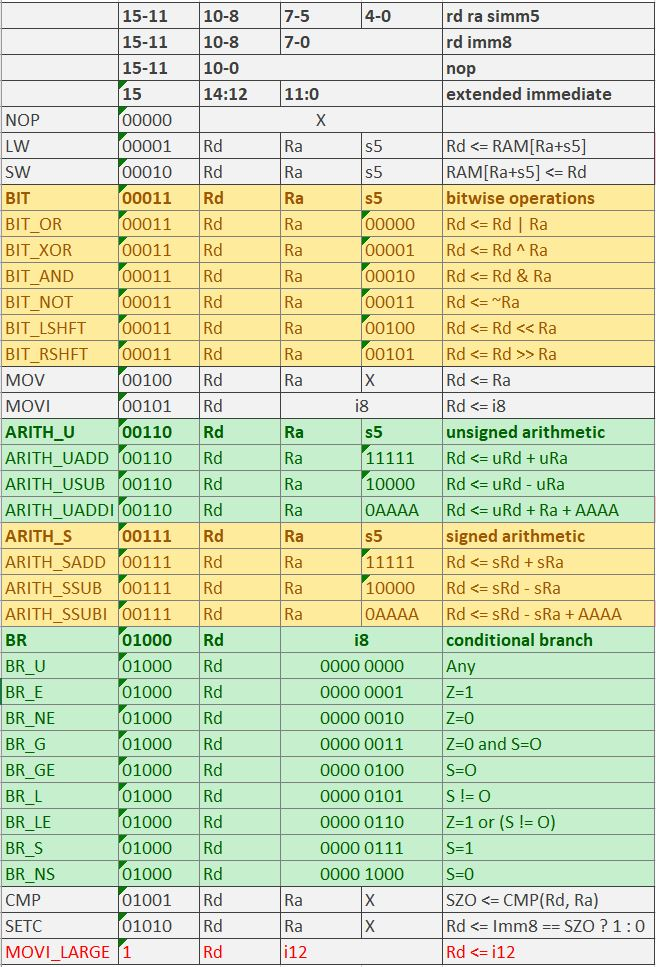
\includegraphics[width=9cm]{../img/isa}
\caption{Initial Vmicro16 16-bit instruction set architecture. Coloured regions represent instruction families (bitwise, branching, arithmetic, etc.).}
\label{fig:isa}
\end{figure}
The ISA table is shown in Figure \ref{fig:isa}. The top 5 bits (15-11) are dedicated to the opcode resulting in 32 unique values. Currently only the bits 14-11 are used (\verb|NOP| to \verb|SETC|) leaving the top bit spare. Initially, this bit was reserved to indicate an extended immediate instruction, \verb|MOVI12|, supporting a large 12-bit immediate value, however later in the design it was decided that the top bit would indicate special instructions dedicated for multi-core operation. This leaves 16 spare unique opcodes for this purpose.


\newpage
\subsection{Design and Implementation}
The RISC core design is a traditional 5-stage processor (fetch, decode, execute, memory, write-back).

To satisfy \ref{cd:vendor}, the Verilog code will be self-contained in a single file. This reduces the hierarchical complexity and eases cross-vendor project set-up as only a single file is required to be included. 
A disadvantage with this single file approach is that some external Verilog verification tools that I plan to use, such as Verilator, do not currently support multiple Verilog modules (due to an unfixed bug) within a single file. 

\subsubsection{Instruction and Data Memory}
The design uses separate instruction and data memories similar to a Harvard architecture computer. This architecture was chosen due to it's simplicity to implement.

\subsubsection{Register File}
To support design goal \ref{isa:regs}, the register set features a dual-port read and single-port write. This allows instructions to read 2 registers simultaneously for any instruction. The single-port write allows the instruction output to be written to the register file. 

\begin{figure}[H]
\centering 
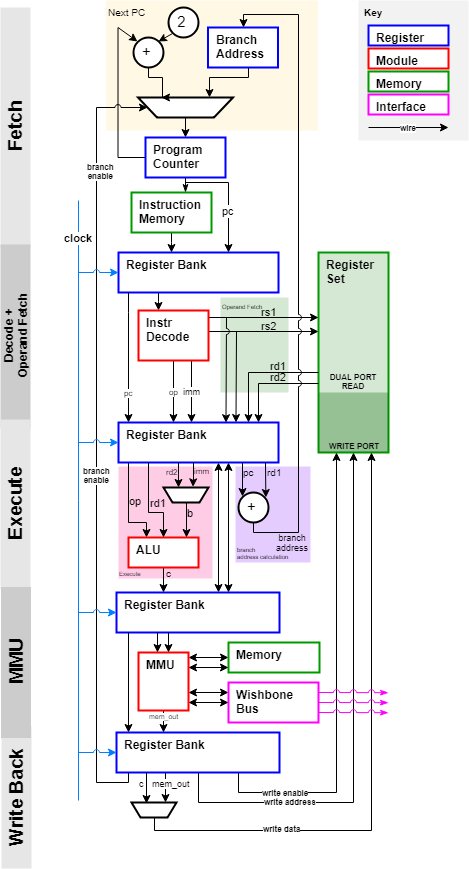
\includegraphics[width=10cm]{../img/risc}
\caption{Vmicro16 RISC 5-stage RTL diagram.}
\label{fig:risc}
\end{figure}

\subsubsection{Pipelining}
The extended deliverable \ref{ed:ipc}, to provide atleast 1 instructions per clock

\begin{figure}[H]
\centering 
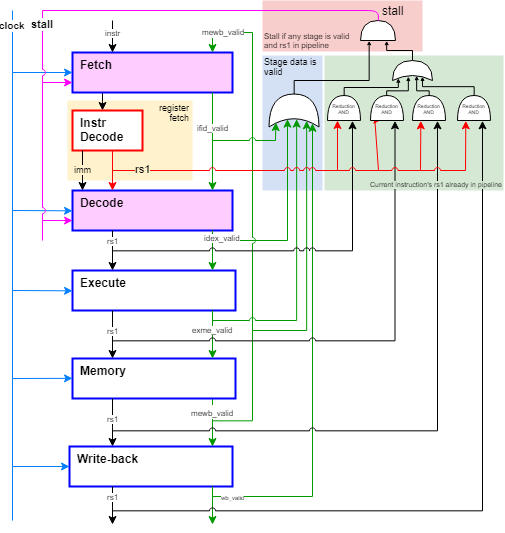
\includegraphics[width=10cm]{../img/stall}
\caption{Pipeline stall detection logic. }
\label{fig:stall}
\end{figure}

\subsubsection{Memory Management Unit}
It was decided to use a memory management unit (MMU) to make it easier and extensible to communicate with external peripherals or additional registers. This method would transparently use the existing \verb|LW|/\verb|SW| instructions which removes the requirement for a unique instruction for each peripheral. 

\subsubsection{Proposed Memory Mapped Addresses}
The proposed memory mapped addresses for each system and peripheral are listed below.

\begin{table}[h]
    \small
    \begin{tabularx}{\textwidth}{|l|X|}
    \hline
    Address (16-bit aligned) & Peripheral Name
    \\ \specialrule{2pt}{-2pt}{0pt}
    \verb|0x0000| & NOP (reads returns 0, writes do nothing)
    \\ \hline 
    \verb|0x00ZZ| & Per-core scratch RAM (ZZ = 8-bit RAM address)
    \\ \hline 
    \verb|0x0100| & Extended Core Registers 1
    \\ \hline 
    \verb|0x0200| & Extended Core Registers 2
    \\ \hline 
    \verb|0x03ZZ| & Wishbone Master controller select (ZZ contains 8-bit wishbone slave address)
    \\ \hline 
    \verb|0x1XYZ| & Master core controller (X = slave select, Y = instruction, Z = data)
    \\ \hline 
    \end{tabularx}
    \caption{Project stages throughout the life cycle of the project.}
    \label{tb:mmu}
\end{table}

\subsubsection{ALU Design}
The Vmicro16's ALU is an asynchronous module that has 3 inputs: data a; data b; and opcode op, and outputs data value c.
The ALU is able to operand on both register data (\verb|rd1| and \verb|rd2|) and immediate values. A switch is used to set the \verb|b| input to either the \verb|rd2| or \verb|imm| value from the previous stage.

Currently, the ALU does not store flags to indicate overflow, equality, or zero values in the module itself. Instead the ALU outputs the result of the \verb|CMP|, which calculates such flags, to be written back to the register set in the write-back stage. This means that in order to perform a conditional operation, such as a branch, the register containing the \verb|CMP| flags must be included in the instruction.

\begin{figure}[H]
\centering 
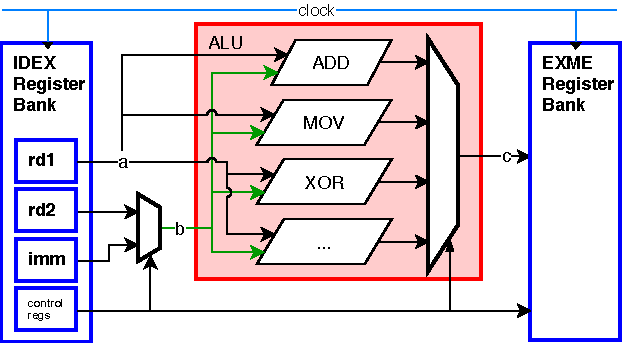
\includegraphics[width=10cm]{../img/alu}
\caption{Vmicro16 ALU diagram showing clocked inputs from the previous IDEX stage being }
\label{fig:alu}
\end{figure}


The Verilog implementation of the ALU is shown in Figure \ref{fig:aluv}. The ALU's asynchronous output is clocked with other registers, such as destination register \verb|rs1| and other control signals, in the \verb|EXME| register bank.
\begin{figure}[H]
\centering
\inputminted[fontsize=\footnotesize,firstline=322,lastline=335,linenos]{verilog}{../../vmicro16/vmicro16.v}
\caption{Vmicro16's ALU implementation named vmicro16\_alu. vmicro16.v}
\label{fig:aluv}
\end{figure}




\subsubsection{Decoder Design}
Instruction decoding occurs in the between the IFID and IDEX stages. 
The decoder extracts register selects and operands from the input instruction. The decoder outputs are asynchronous which allows the register selects to be passed to the register set and register data to be read asynchronously. The register selects and register read data is then clocked into the IDEX register bank.

\begin{figure}[H]
\centering
\inputminted[fontsize=\footnotesize,firstline=224,lastline=245,linenos]{verilog}{../../vmicro16/vmicro16.v}
\caption{Vmicro16's decoder module code showing nested bit switches to determine the intended opcode. vmicro16.v}
\label{fig:decoder}
\end{figure}

In Figure \ref{fig:decoder}, it can be seen that the first 8 opcode cases are represented using the same 15-11 bits, however the \verb|VMICRO16_OP_BIT| instructions require another bit range to be compared to determine the output opcode.

\subsection{Verification}
Currently, the only verification method used is manual inspection of the output waveforms of a test bench.

\subsubsection{Known Bugs}
Several known bugs exist within the RISC core however none are critical as they can be easily avoided in software.

\begin{enumerate}[leftmargin=3\parindent, label=\bfseries BUG\arabic*, style=nextline]
\item{\textbf{Stall detection does not consider load/store instructions.}\\
Due to pipelining techniques used by the processor and lack of address checking in the \verb|EXME| and \verb|MEWB| stages, \verb|LW| instructions immediately after \verb|SW| instructions:\\ \verb|    SW R0 (R2+16)|\\ \verb|    LW R1 (R2+16)|\\
will not return the previously stored value. In addition, because of the target address is calculated by the ALU (e.g. \verb|R2+16|), detecting matching addresses at IFID and IDEX stage is not trivial, and because of this, a hardware fix is not planned for the final version. It is possible to overcome this problem in software by placing at least 5 \verb|NOP| instructions after each \verb|SW|. 
}\label{bug:swlw}
\end{enumerate}


\chapter{Future Progress}

{\hypersetup{linkcolor=black}
\startcontents[chapters]
\printcontents[chapters]{}{1}{}
}
\noindent\\
This chapter discusses planned future work

\section{Project Status}
The project has progresses at an acceptable speed

\begin{table}[h]
    \small
    \begin{tabularx}{\textwidth}{|l|l|l|l|X|}
    \hline
    Stage & Title & Start Date & Core & Status
    \\ \specialrule{2pt}{-2pt}{0pt}
    1.0 & Research & Feb 04 & x & Completed
    \\ \hline
    1.1 & Requirement gathering/review & Feb 11 & x & Completed
	\\ \hline
    1.1 & Processor specification, architecture, ISA & Feb 18 & x & Completed
	\\ \hline
    1.2 & Stage/Time Allocation Planning & Feb 25 & x & Completed
    \\ \specialrule{2pt}{-2pt}{0pt}
    2.1 & Decoder, Register Set, impl \& integration & Feb 25 & x & Completed
	\\ \hline
    2.2 & Register set impl \& integration & Mar 04 & x & Completed
	\\ \hline
    2.3 & Local memory impl \& integration & Mar 11 & x & Completed
    \\ \specialrule{2pt}{-2pt}{0pt}
    3.1 & Memory mapped register layout \& impl & Apr 01 &  & On-going
	\\ \hline
    3.2 & Wishbone peripheral bus connected to MMU & Apr 081 &  & On-going
	\\ \hline
    3.3 & Pipelined implementation and verification & Apr 15 &  & On-going
	\\ \hline
    3.4 & Cache memory design \& impl & Apr 22 &  & Not planned
    \\ \specialrule{2pt}{-2pt}{0pt}
    4.1 & Multi-core communication interface & TBD & x & Planned
	\\ \hline
    4.2 & Shared-memory controller & TBD & x &Planned
	\\ \hline
    4.3 & Scalable multi-core interface (10s of cores) & TBD & x & Planned
	\\ \hline
    4.4 & Multi-core example program (reduction) & TBD & x & Planned
    \\ \specialrule{2pt}{-2pt}{0pt}
    5.1 & SPI-FPGA interface for OTG programming & TBD &  & Unknown
	\\ \hline
    5.2 & FPGA-PC interfacing & TBD &  & Unknown
	\\ \hline
    5.3 & FPGA-PC debugging (instruction breakpoints) & TBD & & Unknown
    \\ \specialrule{2pt}{-2pt}{0pt}
    6.1 & Compiler backend for vmicro16 & TBD &  & Unknown
	\\ \hline
    6.2 & Compiler support for multi-core codegen & TBD &  & Unknown 
    \\ \specialrule{2pt}{-2pt}{0pt}
    7.1 & Wishbone peripherals for demo & TBD & x & Planned
    \\ \specialrule{2pt}{-2pt}{0pt}
    8.1 & Final Report & TBD & x & Planned
	\\ \hline    \end{tabularx}
    \caption{Project stages throughout the life cycle of the project.}
    \label{tb:future_stages}
\end{table}

\subsection{Updated Project Time Line}

\begin{figure}[h]
\centering 
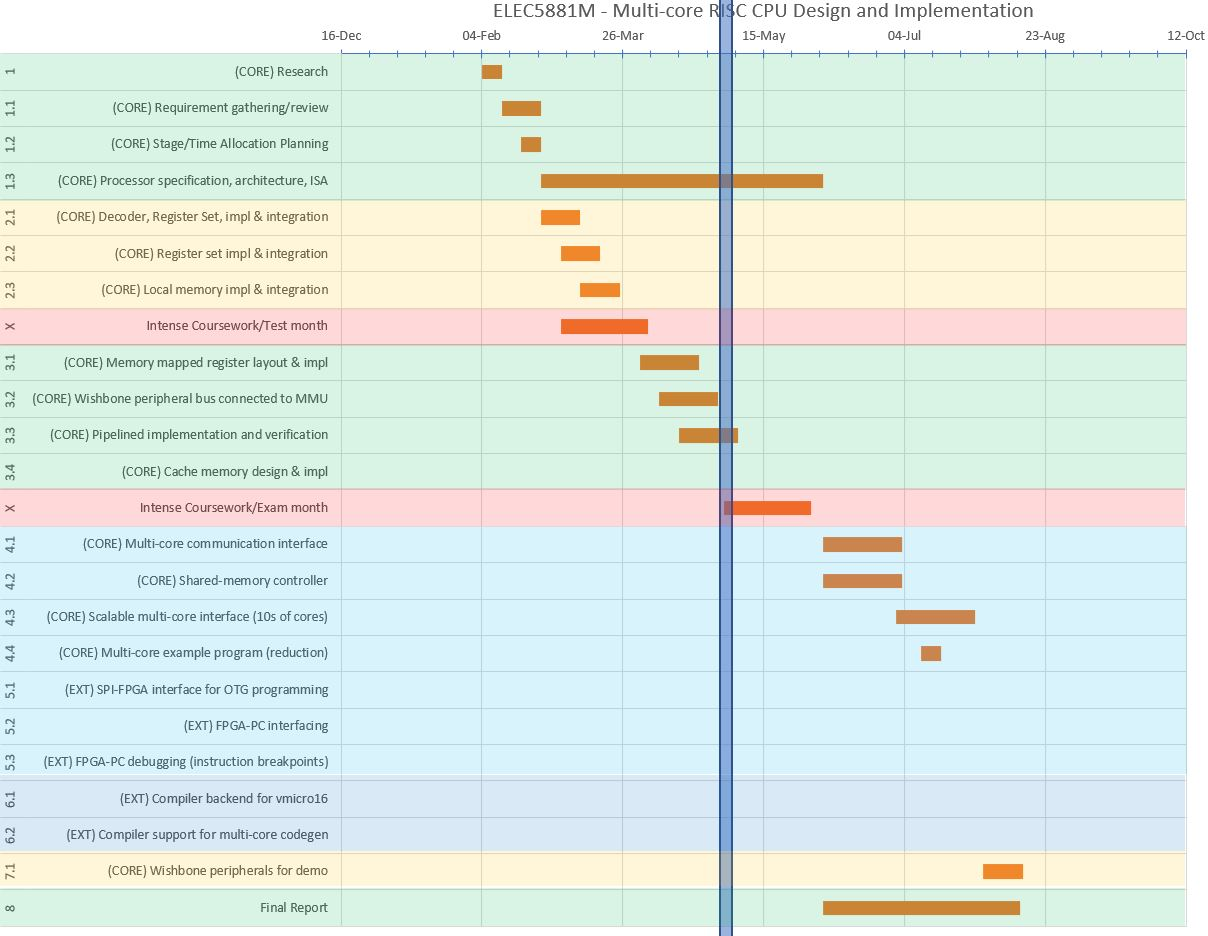
\includegraphics[width=12cm]{../img/week2_gantt}
\caption{Updated project time gantt chart showing time allocations for stage 4.}
\label{fig:week2_gantt}
\end{figure}

\section{Multi-core Functionality}
    \section{Interconnect Goals}
    \section{Interconnect Layout}
        \subsection{Bus Design}
        \subsection{Core Pin Assignments}
    \section{Core-to-core Communication}
    \section{Shared-Resource Control}
        \subsection{Resource Scheduling}
    \section{Verification}
    \section{Conclusion}
    

\newpage
\cite{openpiton}
\cite{satish2009designing}
\cite{binet2010harnessing}
\bibliography{refs}
\addcontentsline{toc}{chapter}{References}

%\chapter{RISC Core Design}
%{\hypersetup{linkcolor=black}
%\startcontents[chapters]
%\printcontents[chapters]{}{1}{}
%}
%    \section{Design Goals}
%    \section{Instruction Set Architecture}
%        \subsection{Data Sizes}
%        \subsection{Registers}
%        \subsection{Endianness}
%    \section{High Level Design}
%    \section{Memory-mapped peripherals}
%        \subsection{Wishbone Master Bus}
%    \section{Optimisations}
%        \subsection{Pipelining}
%        \subsection{Stall Avoidance}
%    \section{Core Verification}
%    \section{Conclusion}
%        
%\chapter{Multi-core Communication Design}
%{\hypersetup{linkcolor=black}
%\startcontents[chapters]
%\printcontents[chapters]{}{1}{}
%}
%    \section{Interconnect Goals}
%    \section{Interconnect Layout}
%        \subsection{Bus Design}
%        \subsection{Core Pin Assignments}
%    \section{Core-to-core Communication}
%    \section{Shared-Resource Control}
%        \subsection{Resource Scheduling}
%    \section{Verification}
%    \section{Conclusion}
%
%\chapter{Core Analysis}
%{\hypersetup{linkcolor=black}
%\startcontents[chapters]
%\printcontents[chapters]{}{1}{}
%}
%    \section{FPGA Implementation Analysis}
%        \subsection{Space/Resource Usage}
%        \subsection{Static Timing Analysis}
%    \section{Speed Analysis}
%        \subsection{Parallel Reduction Algorithms}
%        \subsection{Parallel DFT Algorithm}
%
%
%\chapter{Conclusion}
%{\hypersetup{linkcolor=black}
%\startcontents[chapters]
%\printcontents[chapters]{}{1}{}
%}
%    \section{RISC Core Review}
%    \section{Multi-core Review}
%    \section{Verification Review}
%    \section{Goal Review}

%
%\chapter*{Preface}
%\label{sect:preface}
%This report discusses the design, implementation, and verification, of an FPGA-based embedded processor (processor) and compiler.
%
%
%A field-programmable gate array (FPGA) is a reprogrammable logic device that enables digital electronic designs to be realised and executed on-chip. FPGAs utilise configurable logic blocks (CLB) that can be configured to emulate primitive gates. Connecting these primitive gates with others allows the engineer to realise complex logic such as combinational gates, multiplexers, and lookup-tables. Modern FPGA devices also include components such as block-RAMs, DLLs, and DSP blocks.
%
%An embedded processor will be designed using the Verilog hardware description language (HDL). A HDL can be thought of as a front-end to a software compiler. Other HDL front-ends exist such as VHDL. The HDL is synthesised into an retargetable intermediate form consisting of nets - a form describing the gates, flip-flops, and their interconnections. After this synthesis takes place, the intermediate net list form is transformed into implementation specific forms. As this processor is designed for FPGA implementation, processes such as "place and route" are utilised to map the net list to physical resources on the FPGA. Different processes are performed for different implementations, such as for ASICs and CPLDs.
%
%\newpage
%\chapter{RISC Machines}
%{%\hypersetup{linkcolor=black}
%\startcontents[chapters]
%\printcontents[chapters]{}{1}{}
%}
%
%\section{Introduction}
%\lipsum[1]
%
%This \mintinline{c}{
%int main(int argc, char** argv);
%} is the.
%
%\begin{figure}[H]
%\centering
%\mintinline{c}{
%int main(int argc, char** argv);
%}
%\caption{Foo bar}
%\end{figure}
%\lipsum[2]
%
%\section{Background}
%\lipsum[1-2]
%\subsection{Soft-core Embedded Processors}
%\lipsum[1-2]
%\subsection{Compilers}
%\lipsum[1-2]
%\section{Project Overview}
%\lipsum[1-2]
%
%This \mintinline{c}{
%int main(int argc, char** argv);
%} is the.
%
%\begin{figure}[H]
%\centering
%\mintinline{c}{
%int main(int argc, char** argv);
%}
%\caption{Foo bar}
%\end{figure}

\end{document}